\documentclass[11pt,a4paper]{article}

\newcommand{\tumsoTime}{09:00 น. - 12:00 น.}
\newcommand{\tumsoRound}{1}

\usepackage{../tumso}

\begin{document}

\begin{problem}{Tetris Battle 2}{standard input}{standard output}{1.5 seconds}{512 megabytes}{200}

ย้อนกลับไปในการแข่งขัน Tetris Battle ครั้งที่ 1 เรื่องราวมีอยู่ว่า Tetris เกมต่อบล็อกขนาด $4$ หน่วยที่ทุกคนคุ้นเคย ถ้าคิดภาพไม่ออกก็ตามภาพ ... ด้านบนมาแปลงเพื่อปั่น ToroTN อีกทีว่า (สามารถติดตามเรื่องราวได้ที่ \textcolor{blue}{\href{https://api.otog.cf/problem/doc/844}{Tetris Battle})}

โดยในการแข่งขัน Tetris Battle ครั้งที่ 2 นี้ จะเป็นการแข่งวางบล็อก Tetris ที่ไม่ได้มีแค่ใน Tetris (นั่นคือเป็นรูปแบบใด ๆ ก็ได้) โดยจะมีแถวในเกมนี้ทั้งหมด $N$ คอลัมน์ โดยที่ เริ่มต้นจะมีความสูงของบล็อกในช่องที่ $i$ ที่วางอยู่แล้วเท่ากับ $A_i$

ตัวอย่างเช่น ถ้า $N=7$ และ $A_1=2,A_2=5,A_3=1,A_4=7,A_5=4,A_6=3,A_7=6$ ตารางของ Tetris ที่ถูกวางแล้วจะมีลักษณะเป็นดังรูป
\begin{center}
\parindent \resizebox{3cm}{!}{
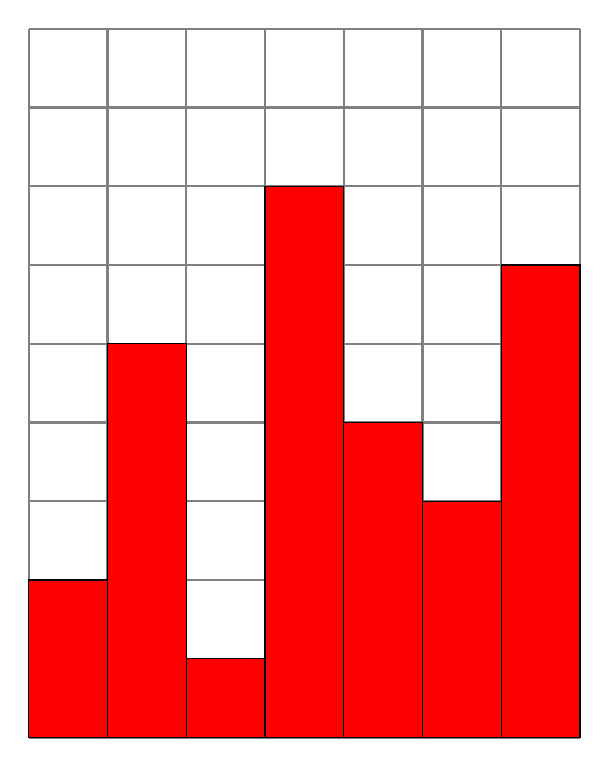
\begin{tikzpicture}
    \draw[step=1cm,gray,thick] (0.0,0.0) grid (7.0,9.0);
    \filldraw[fill=red,draw=black] (0,0) rectangle (1,2);
    \filldraw[fill=red,draw=black] (1,0) rectangle (2,5);
    \filldraw[fill=red,draw=black] (2,0) rectangle (3,1);
    \filldraw[fill=red,draw=black] (3,0) rectangle (4,7);
    \filldraw[fill=red,draw=black] (4,0) rectangle (5,4);
    \filldraw[fill=red,draw=black] (5,0) rectangle (6,3);
    \filldraw[fill=red,draw=black] (6,0) rectangle (7,6);
\end{tikzpicture}
}
\end{center}

Leomotors ผู้เล่นมือใหม่ในการแข่งขัน Tetris ต้องการจะชนะผู้ที่ครองแชมป์มายาวนานอย่าง ToroTN ดังนั้นเขาจึงต้องการทราบว่าเขาสามารถลงชิ้นบล็อกปัจจุบันได้ไหม แต่ด้วยความที่เขาต้องการอยากจะชนะมากจึงต้องการความช่วยเหลืออยู่ทั้งหมด $Q$ โดยในคำถามที่ $i$ Leomotors จะให้ความยาวของชิ้นบล็อกเท่ากับ $S_i$ และบอกว่าแต่ละชิ้นมีรูปร่างอย่างไร โดยบอกเป็นความยาวจากแนวระดับ เรียงทีละคอลัมน์ของบล็อก $B_{i,1},B_{i,2},\ldots,B_{i,S_i}$

ตัวอย่างเช่น ถ้าบล็อกยาว $S_i=5$ และ $B_{i,1}=3,B_{i,2}=6,B_{i,3}=2,B_{i,4}=5,B_{i,5}=4$ จะมีลักษณะของบล็อกดังรูป
\begin{center}
\parindent \resizebox{3cm}{!}{
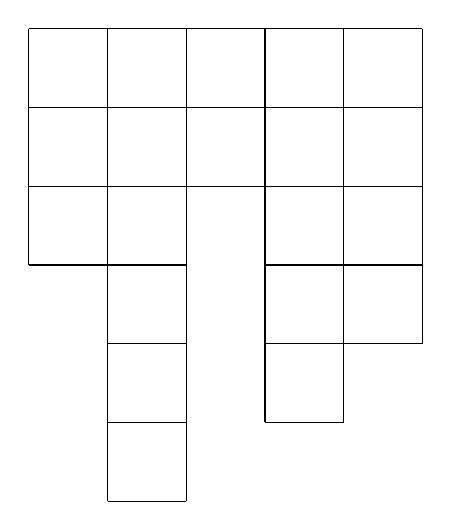
\begin{tikzpicture}
    \draw[step=1cm,white,thick] (0.0,0.0) grid (5.0,6.0);
    \filldraw[draw=black] (0,3) grid (1,6);
    \filldraw[draw=black] (1,0) grid (2,6);
    \filldraw[draw=black] (2,4) grid (3,6);
    \filldraw[draw=black] (3,1) grid (4,6);
    \filldraw[draw=black] (4,2) grid (5,6);
\end{tikzpicture}
}
\end{center}

เพื่อให้เขาสามารถคิดกลยุทธที่ดีที่สุดได้ เขาจึงอยากรู้จำนวนวิธีที่เขาสามารถวางบล็อกดังกล่าวได้ ซึ่งจำนวนวิธีจะนับเป็นหนึ่งวิธีก็ต่อเมื่อวางบล็อกลงไปแล้วไม่เหลือช่องว่างระหว่างบล็อกที่วางลงไปกับบล็อกที่มีอยู่

ตัวอย่างเช่น

\begin{center}
\parindent \resizebox{3cm}{!}{
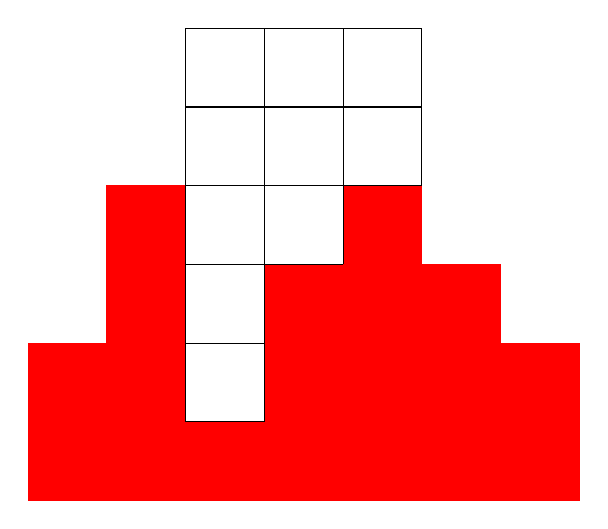
\begin{tikzpicture}
    \filldraw[fill=red,draw=red] (0,0) rectangle (1,2);
    \filldraw[fill=red,draw=red] (1,0) rectangle (2,4);
    \filldraw[fill=red,draw=red] (2,0) rectangle (3,1);
    \filldraw[fill=red,draw=red] (3,0) rectangle (4,3);
    \filldraw[fill=red,draw=red] (4,0) rectangle (5,4);
    \filldraw[fill=red,draw=red] (5,0) rectangle (6,3);
    \filldraw[fill=red,draw=red] (6,0) rectangle (7,2);
    \filldraw[draw=black] (2,1) grid (3,6);
    \filldraw[draw=black] (3,3) grid (4,6);
    \filldraw[draw=black] (4,4) grid (5,6);
\end{tikzpicture}
}
\end{center}

จะเป็นการประกบที่พอดีซึ่งนับว่าเป็นจำนวนหนึ่งวิธีที่สามารถวางบล็อกได้

แต่ถ้าเป็นรูปแบบ

\begin{center}
\parindent \resizebox{3cm}{!}{
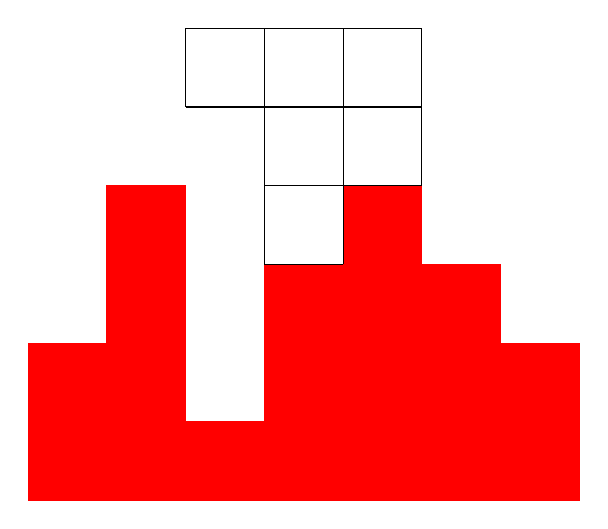
\begin{tikzpicture}
    \filldraw[fill=red,draw=red] (0,0) rectangle (1,2);
    \filldraw[fill=red,draw=red] (1,0) rectangle (2,4);
    \filldraw[fill=red,draw=red] (2,0) rectangle (3,1);
    \filldraw[fill=red,draw=red] (3,0) rectangle (4,3);
    \filldraw[fill=red,draw=red] (4,0) rectangle (5,4);
    \filldraw[fill=red,draw=red] (5,0) rectangle (6,3);
    \filldraw[fill=red,draw=red] (6,0) rectangle (7,2);
    \filldraw[draw=black] (2,5) grid (3,6);
    \filldraw[draw=black] (3,3) grid (4,6);
    \filldraw[draw=black] (4,4) grid (5,6);
\end{tikzpicture}
}
\end{center}

จะประกบกันไม่พอดีจึงไม่นับเป็นวิธีที่สามารถวางบล็อก

\InputFile
ข้อมูลนำเข้ามีทั้งหมด $Q+3$ บรรทัด

บรรทัดแรกประกอบด้วยจำนวนเต็ม $N$ แทนจำนวนคอลัมน์ของ Tetris $(1\leq N,Q\leq 10^{6})$

บรรทัดที่ $2$ ประกอบด้วยจำนวนเต็ม $N$ จำนวน คือ $A_1,A_2,\ldots,A_N$ โดยที่ $A_i$ แทนความสูงของบล็อกที่วางอนู่แล้วในช่องที่ $i$ $(1\leq A_i\leq 10^{18})$

บรรทัดที่ $3$ ประกอบด้วยจำนวนเต็ม $Q$ แทนจำนวนคำถาม โดยที่คำถามแต่ละคำถามไม่เกี่ยวข้องกัน

อีก $Q$ บรรทัดประกอบด้วยจำนวนเต็ม $S_i$ อีก $S_i$ จำนวน คือ $B_{i,1},B_{i,2},\ldots,B_{i,S_i}$ โดยที่ $B_{i,j}$ แทน ความสูงวัดจากแนวระดับ $(1\leq S_i\leq N,1\leq B_{i,j}\leq 10^{18})$

รับประกันว่า $\sum\limits_{i=1}^nS_i\leq 5\cdot 10^5$

\OutputFile
มีทั้งหมด $Q$ บรรทัด ซึ่งบรรทัดที่ $i$ แสดงถึงจำนวนวิธีที่สามารถวางบล็อกที่ $i$ ได้

\Scoring
ชุดทดสอบจะถูกแบ่งเป็น 2 ชุด จะได้คะแนนในแต่ละชุดก็ต่อเมื่อโปรแกรมให้ผลลัพธ์ถูกต้องในชุดทดสอบย่อยทั้งหมด

\begin{description}

\item[ชุดที่ 1 (9 คะแนน)] จะมี $1\leq S_i\leq 2$
\item[ชุดที่ 2 (17 คะแนน)] จะมี $1\leq S_i\leq 4$
\item[ชุดที่ 3 (27 คะแนน)] จะมี $1\leq S_i\leq 10$
\item[ชุดที่ 4 (48 คะแนน)] จะมี $1\leq N,Q\leq 1000$
\item[ชุดที่ 5 (99 คะแนน)] ไม่มีเงื่อนไขเพิ่มเติม 

\end{description}

\Examples

\begin{example}
\exmp{10
4 2 1 3 1 3 1 3 2 3
2
2 1 2
3 2 4 2
}{2
2
}%
\end{example}

\Note

คำอธิบายคำถามที่ 1\\
สามารถวางได้ทั้งหมด $2$ แบบ คือวางในตำแหน่งที่ $2$ $3$ และ $8$ $9$

คำอธิบายคำถามที่ 2\\
สามารถวางได้ทั้งหมด $2$ แบบ คือวางในตำแหน่ง $4$ $5$ $6$ และ $6$ $7$ $8$

\end{problem}

\end{document}
